% !TEX options=--shell-escape
\documentclass[usenames,dvipsnames,9pt]{beamer}

\usepackage{tikz}
\usetikzlibrary{arrows,shapes,snakes,automata,calc,matrix,backgrounds,petri, positioning}

\makeatletter
\def\input@path{{../support/beamer-template/}}
\makeatother

\usepackage{../support/beamer-template/beamerthememetropolis}

\usepackage[utf8]{inputenc}
\usepackage[czech]{babel}
\selectlanguage{czech}

\usepackage{hyperref}
\usepackage{fontawesome}
\usepackage{minted}
\usepackage{mathtools}
\usepackage{tabularx}
\usepackage{smartdiagram}
\usepackage{soul}
\usepackage{tikz}
\usepackage{amssymb}
\usepackage{qrcode}

% Commands shared between most of the tutorial slides

% Homework deadlines
\newcommand{\hwVIIdeadline}{10. 5. 2020}



% Download icon and text with link relative to the root of the courseware site
\newcommand{\download}[1]{\hfill\faDownload\hspace{5pt}\href{https://cw.fel.cvut.cz/wiki/_media/courses/be4m36mas/#1}{\tt #1}\\[1.3em]}

% Draw eye icon
\newcommand{\see}[1]{\faEye\hspace{5pt}#1}

\newcommand{\sep}{\hspace{10pt}/\hspace{10pt}}

\def\Ipe#1{\def\IPEfile{#1}\input{#1}}

% Draw pacman icon
\newcommand{\pacman}[1]{\tikz[baseline=.1em,scale=.6]{
    \useasboundingbox (.02,0) rectangle (.6,.6);
  \draw [fill=#1] (.3,.3) -- ++(25:.3) arc (+25:+335:.3) -- cycle;

}}

% Draw ghost icon
\newcommand{\ghost}[1]{\tikz[baseline=.1em,scale=.5]{
  \draw [fill=#1] (0,0) -- (0,.5) arc (+180:0:.3) -- (.6,0) --
  (.5,.15) -- (.4,0) -- (.3,.15) -- (.2,0) -- (.1,.15) -- cycle;
    \coordinate (eye) at (360*rand:.03);
    \foreach \x in {.17,.43}{
      \fill[white] (\x,.5) circle[radius=.1];
      \fill[black] (\x,.5) ++(eye) circle[radius=.05];
    }
}}

\newcommand{\desc}[2]{
  #1

  \vspace{-0.6em}
  \hfill\begin{minipage}{0.9\linewidth}
    #2
  \end{minipage}

  \vspace{0.2em}
}

\newcommand{\redc}{\tikz\draw[red,fill=red] (0,0) circle (.5ex);}

\newcommand{\greenc}{\tikz\draw[green,fill=green] (0,0) circle (.5ex);}


% Default url for generating QR code with feedback form.
\newcommand{\defaultfeedbackurl}{https://forms.gle/vwbWazEu14w1Kf487}

% Generate frame with QR code to a feedback form.
\newcommand{\framefeedback}[1][\defaultfeedbackurl]{
  \begin{frame}[standout]
    \begin{minipage}{0.4\linewidth}
      \begin{center}
        \textbf{\LARGE Díky za pozornost!}
      \end{center}

      \vspace{3em}

      \raggedleft\small Budeme rádi za Vaši\\zpětnou vazbu! $\rightarrow$
    \end{minipage}
    \hfill
    \begin{minipage}{0.5\linewidth}
      \vspace{4em}
      \centering\qrcode[height=\linewidth]{#1}\\
      \vspace{0.8em}
      \url{#1}
    \end{minipage}
  \end{frame}
}

\title{Úvod do distribuovaných výpočtů}
\date{}
\institute{B4B36PDV -- Paralelní a distribuované výpočty}

\metroset{block=fill}

\begin{document}
\maketitle

\begin{frame}
  \frametitle{Osnova}
  \begin{itemize}
    %\item Opakování z minulého cvičení\\[1.5em]
    \item Distribuovaný výpočet
    \item DSand framework
    \item Distribuované prohledávání%\\[1.5em]
  \end{itemize}
\end{frame}


%\section{Opakování z minulého cvičení}
%
%\begin{frame}[standout]
%  \Huge
%  \url{http://goo.gl/a6BEMb}
%\end{frame}
%
%{\setbeamertemplate{frame footer}{\see{\url{http://goo.gl/a6BEMb}}}
%\begin{frame}[fragile]
%\frametitle{Který způsob je efektivnější?}
%
% \begin{minted}{c}
%bool mat[M][N];
% \end{minted}
%
%\end{frame}
%
%\begin{frame}[fragile]
%\frametitle{Jakým způsobem bude následující kód proveden?}
%
% \begin{minted}{c}
%std::cout << "Finished!" << std::endl;
% \end{minted}
%
% \vspace{.3em}
%
% \begin{itemize}
% \item MOZNOST A
% \end{itemize}
%
%\end{frame}
%}

\begin{frame}[standout]
  \begin{center}
    \LARGE Vyžadujeme \textbf{samostatnou} práci na všech úlohách.
  \end{center}

  \vspace{2em}

  \faWarning \hspace{3pt}
  \textbf{Plagiáty jsou zakázané.} Nepřidělávejte prosím starosti nám, ani sobě.
\end{frame}

% \begin{frame}
%   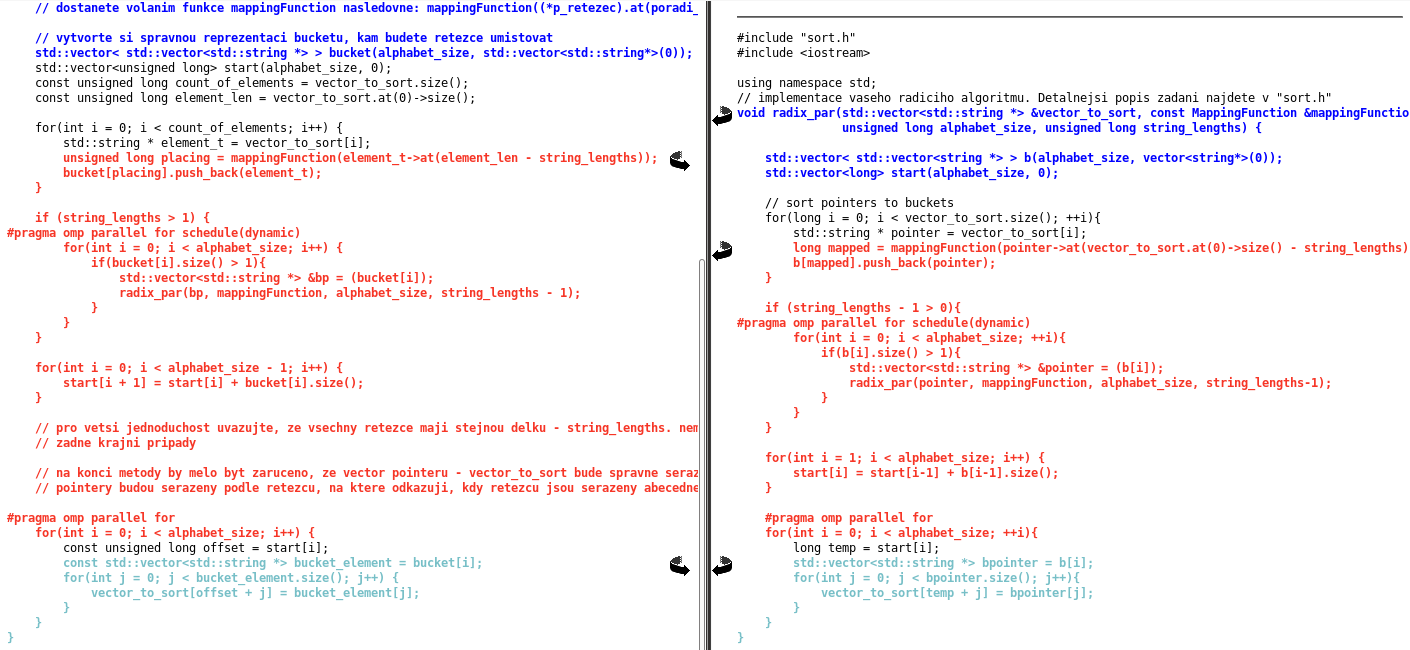
\includegraphics[width=\linewidth]{figs/jplag.png}
% \end{frame}
%
% \begin{frame}[standout]
%   \LARGE\faWarning \hspace{3pt} Pokud se poznáváte (respektive víte, že jste na některé úloze spolupracovali s kolegou v míře větší než malé), tak se nám raději \underline{ozvěte včas}!
% \end{frame}

\section{Distribuovaný výpočet}

\begin{frame}
\frametitle{Moderní procesor}
  \centering
  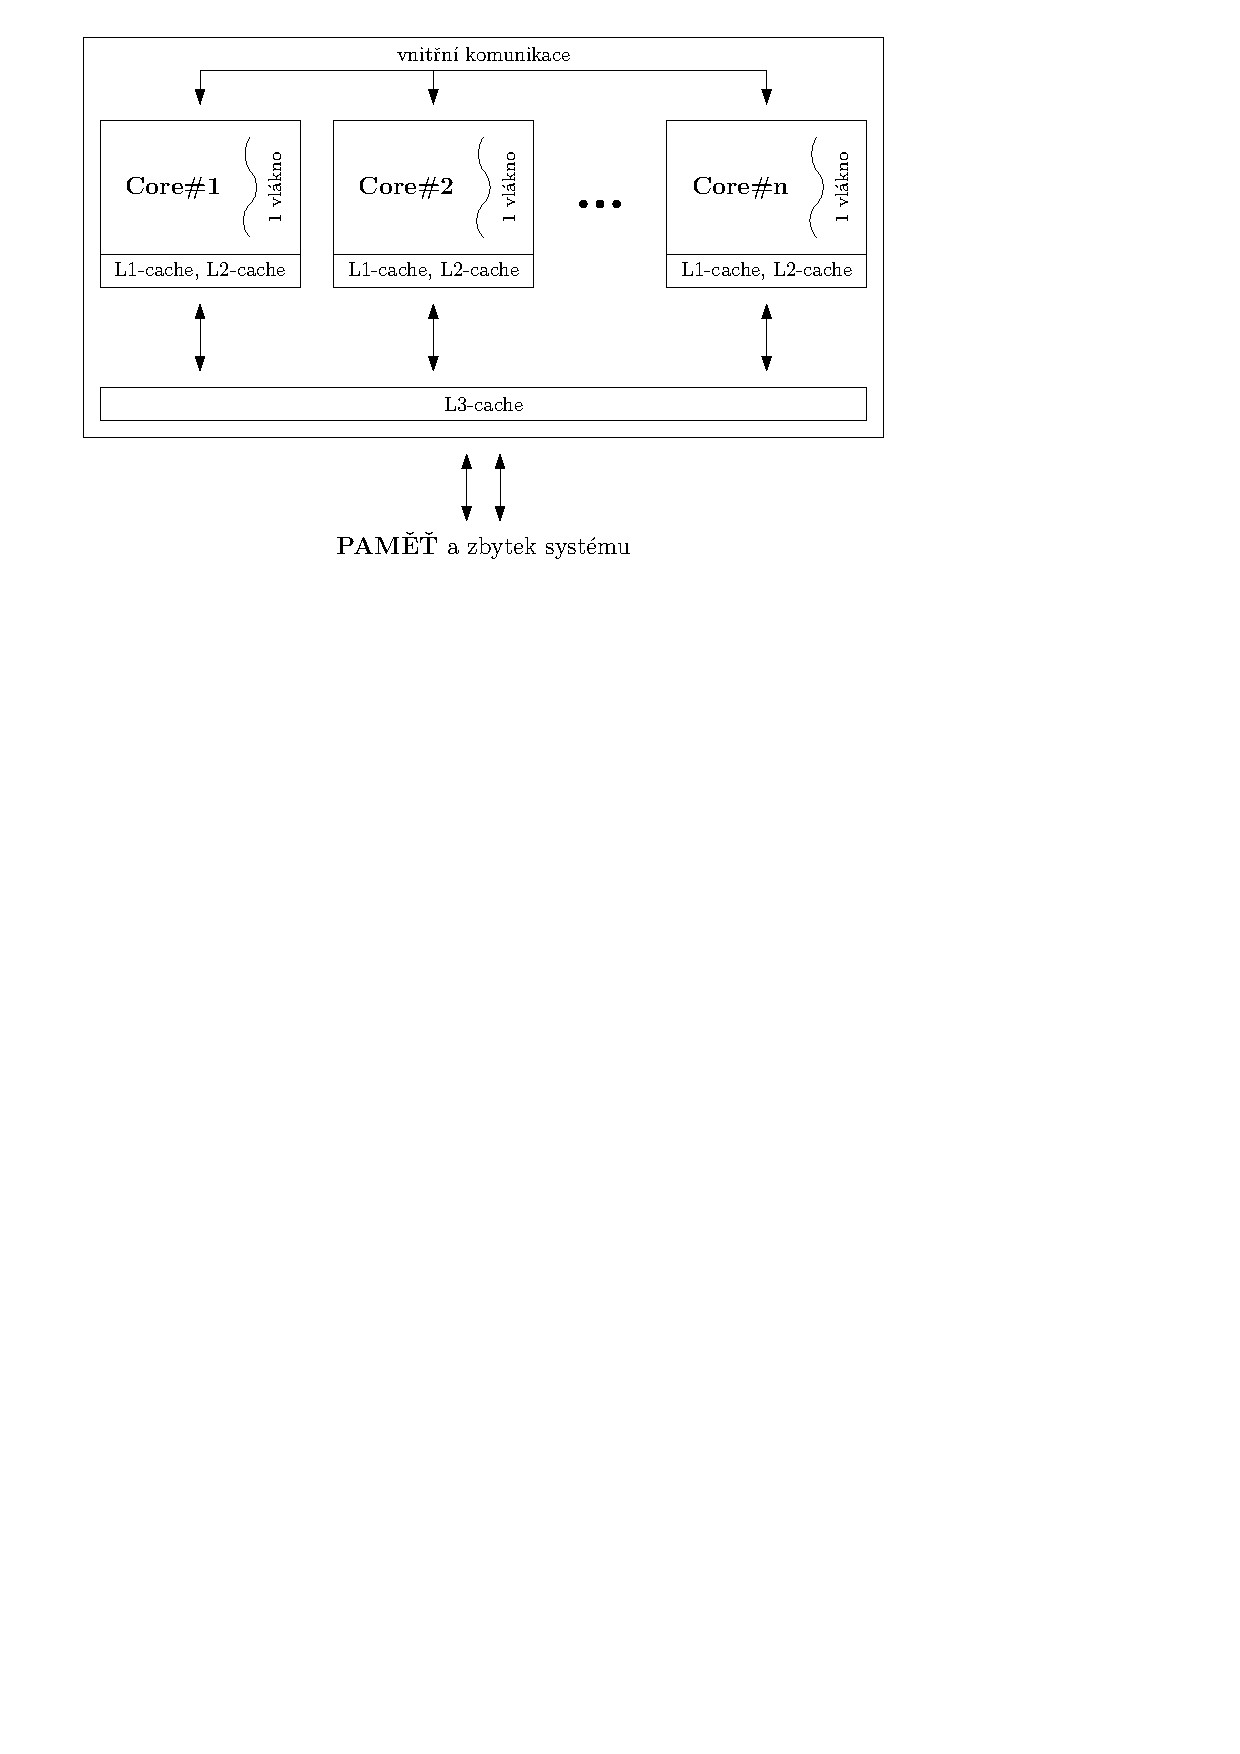
\includegraphics[width=0.8\linewidth]{../../01/tutorial/figs/modern_cpu.pdf}

  \pause\vspace{1.5em}
  \Large Proč bychom mohli chtít tento model opustit?

%An algorithm is parallel if there are several processes (tasks, threads, processors) working on it at the same time. Often the tasks run in the same address space, and can communicate/reference results by others freely (low cost).

%An algorithm is distributed if it is parallel and the tasks run on separate machines (separate address spaces), one task has no direct access to the work of the others. It has to request needed data, or just wait until it is sent to it.
\end{frame}

\begin{frame}
  \frametitle{Motivace distribuovaného výpočtu}

  \begin{itemize}
    \pause\item I ty nejšílenější procesory mají omezený počet vláken (za šílenou cenu) \\
                {\small (Xeon Platinum 9282, 112 vláken, $\sim$\$25000-\$50000 ? (2018))}

    \pause\item Přístupy do sdílené paměti jsou drahé \\
                {\small (I pokud nepotřebujeme synchronizovat! -- sběrnice má omezenou kapacitu)} \\[1.25em]

    \pause\item Jediný ,,stroj`` je \emph{single point of failure} \\
                {\small (Pokud nám selže, tak jsme v háji)}

    \pause\item Chceme být geograficky blíže cílovým uživatelům \\
                {\small (Nižší latence, ...)}
    \pause\item ,,Důvěryhodnost`` výpočtu \\
                {\small (Pokud nám výpočet zverifikuje několik \emph{nezávislých} strojů, je pravděpodobně správný)}
  \end{itemize}
\end{frame}

\begin{frame}
\begin{center}
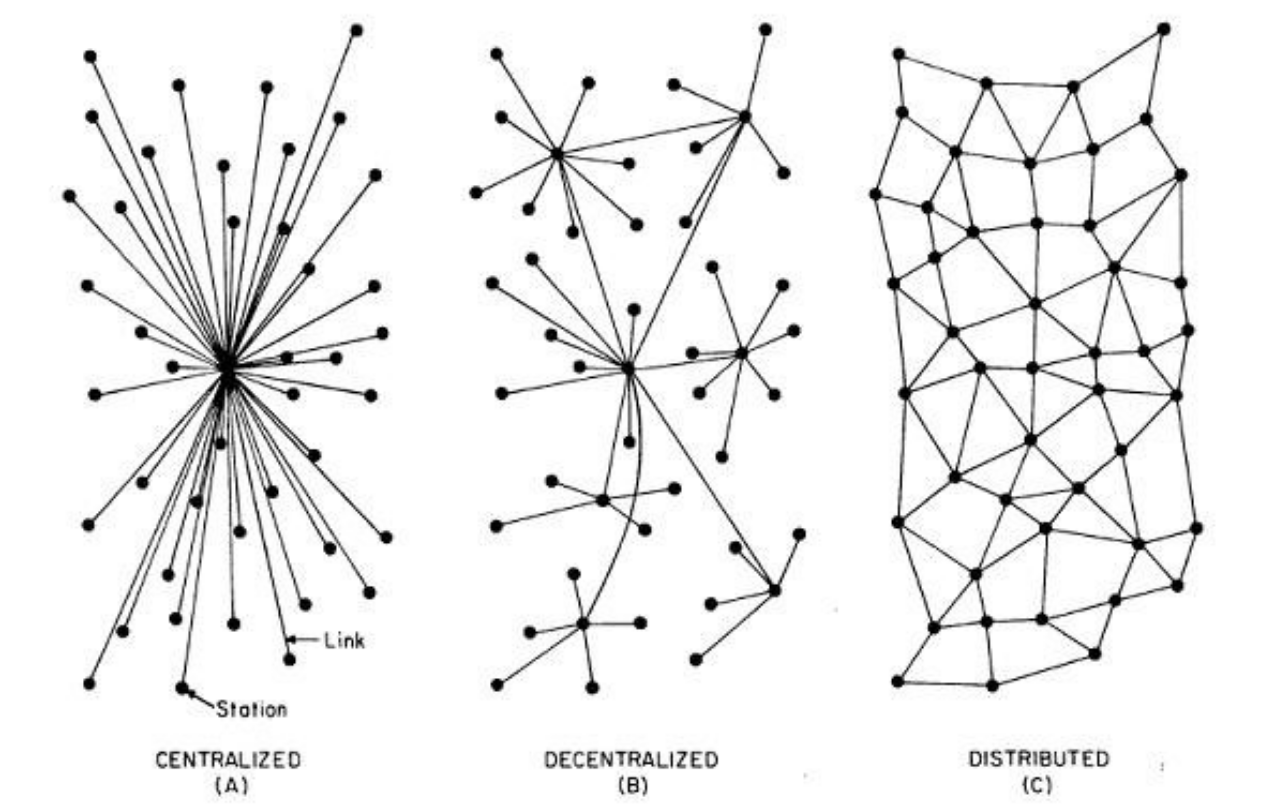
\includegraphics[width=.9\linewidth]{figs/ds.jpeg}
\end{center}
\end{frame}

\begin{frame}
\begin{center}
  
\includegraphics[width=0.4\linewidth]{figs/complete.pdf}
\end{center}
\end{frame}

\begin{frame}

  \begin{center}
    \LARGE Na jaké problémy ale narazíme?
  \end{center}

  \pause\vspace{1em}\hrule\vspace{1em}

  \begin{itemize}
    \item Nespolehlivá komunikace (ztracené/zpožděné zprávy)
    \item Nespolehlivé výpočetní jednotky (musíme počítat se selháním procesu)
  \end{itemize}

  \pause\vspace{0.8em}
  A v nejhorším případě až:
  \begin{itemize}
    \item Zprávy doručené v chybném pořadí (UDP vs. TCP)
    \item Poškozené zprávy
    \item Procesy, které se nás snaží cíleně podvést (například, infikované uzly)
  \end{itemize}

\end{frame}


\begin{frame}
\begin{block}{Čím se budeme zabývat?}
      \begin{itemize}
        \item Výpočet provádí současně více oddělených výpočetních uzlů\\
              {\small (často i geograficky -- my budeme ale distribuovanost simulovat)} \\[1em]
        \item Cíle:
              \begin{itemize}
                \item Zrychlit výpočet
                \item \only<1>{Robustnost výpočtu}
                      \only<2->{\alert{Robustnost výpočtu}}
              \end{itemize}\vspace{1em}
        \item {\small (5 týdnů)}
      \end{itemize}
    \end{block}

  \begin{block}{Úlohy z distribuované části \normalfont(min. 9 bodů)}
    \begin{itemize}
      \item 2 malé úlohy                 \hfill  4 body
      \item Semestrální práce            \hfill 14 bodů
    \end{itemize}
  \end{block}
\end{frame}

\begin{frame}
\frametitle{DSand framework}
  \begin{center}
    \only<1>{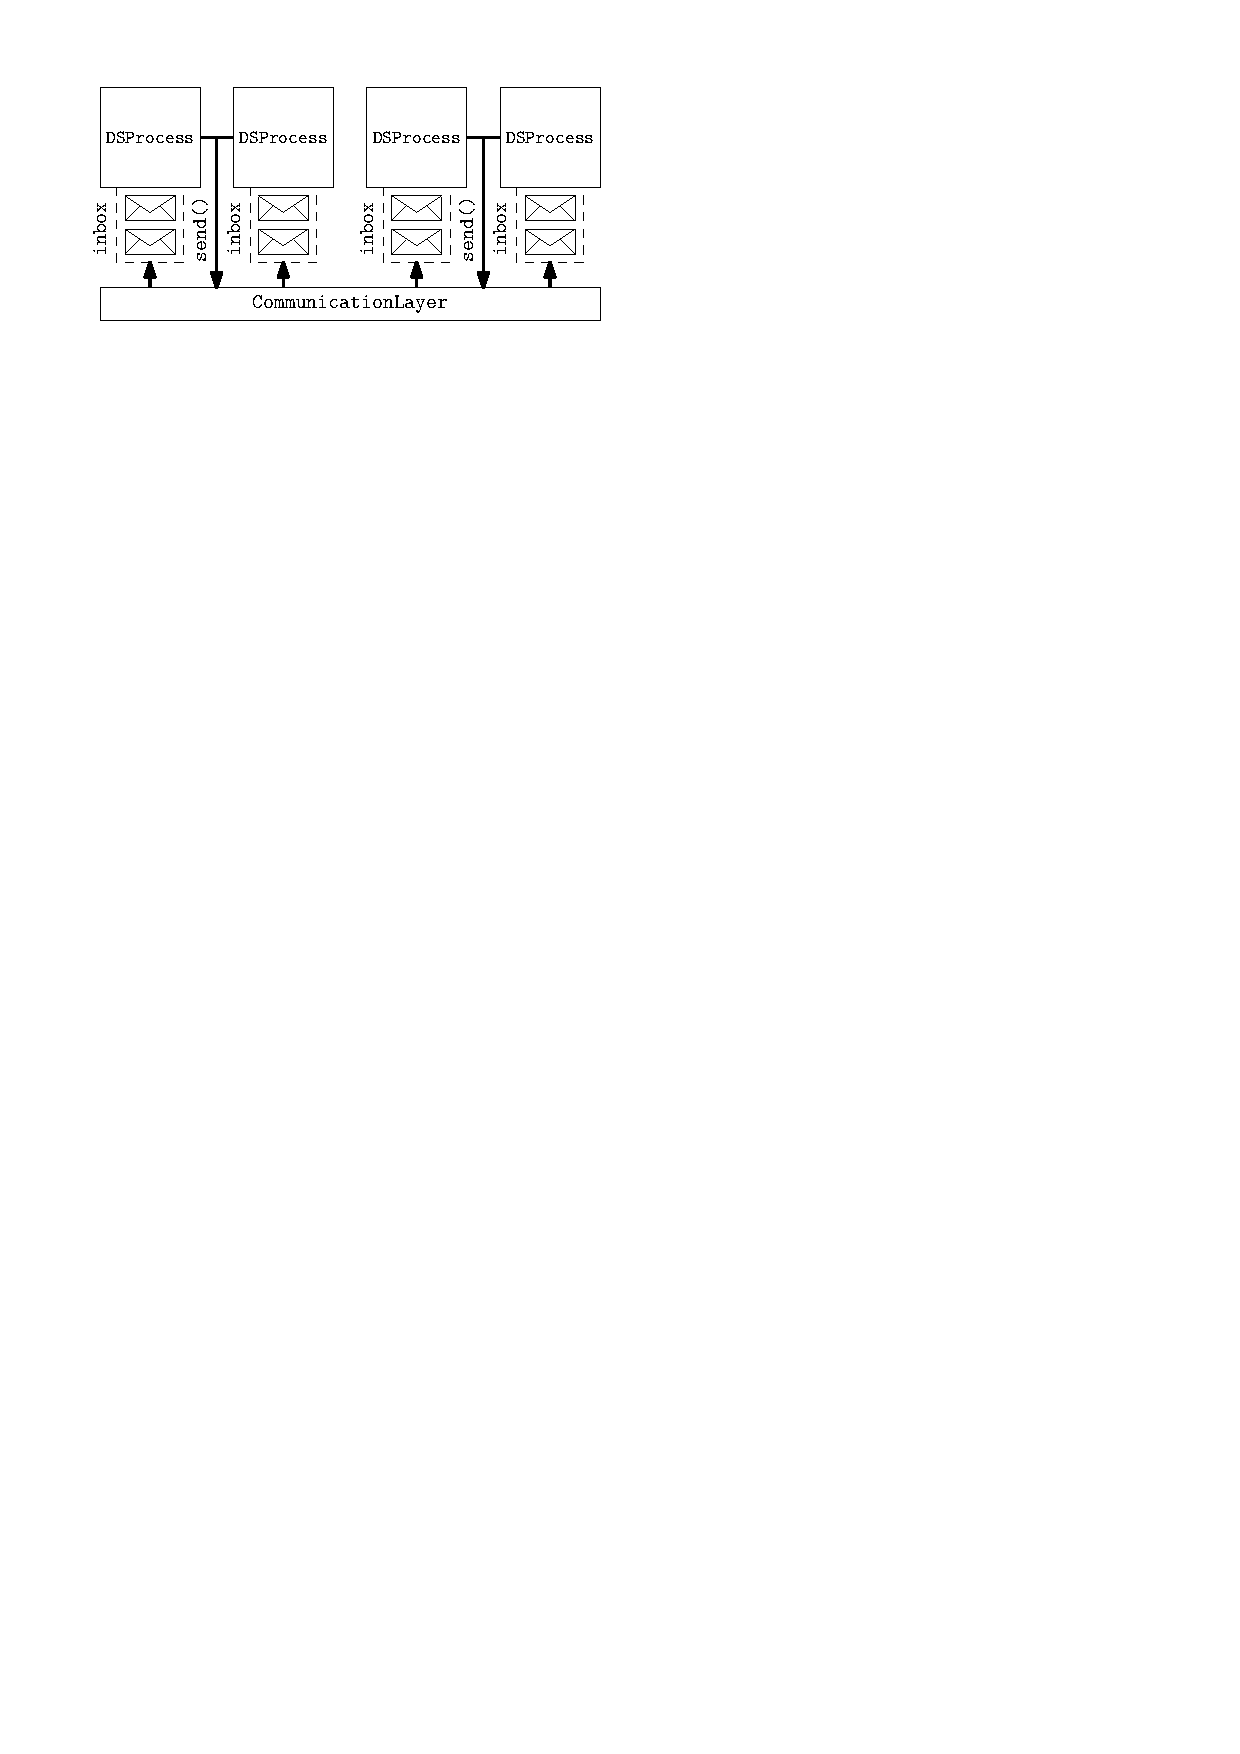
\includegraphics[width=0.9\linewidth]{figs/dsand1.pdf}}%
    \only<2>{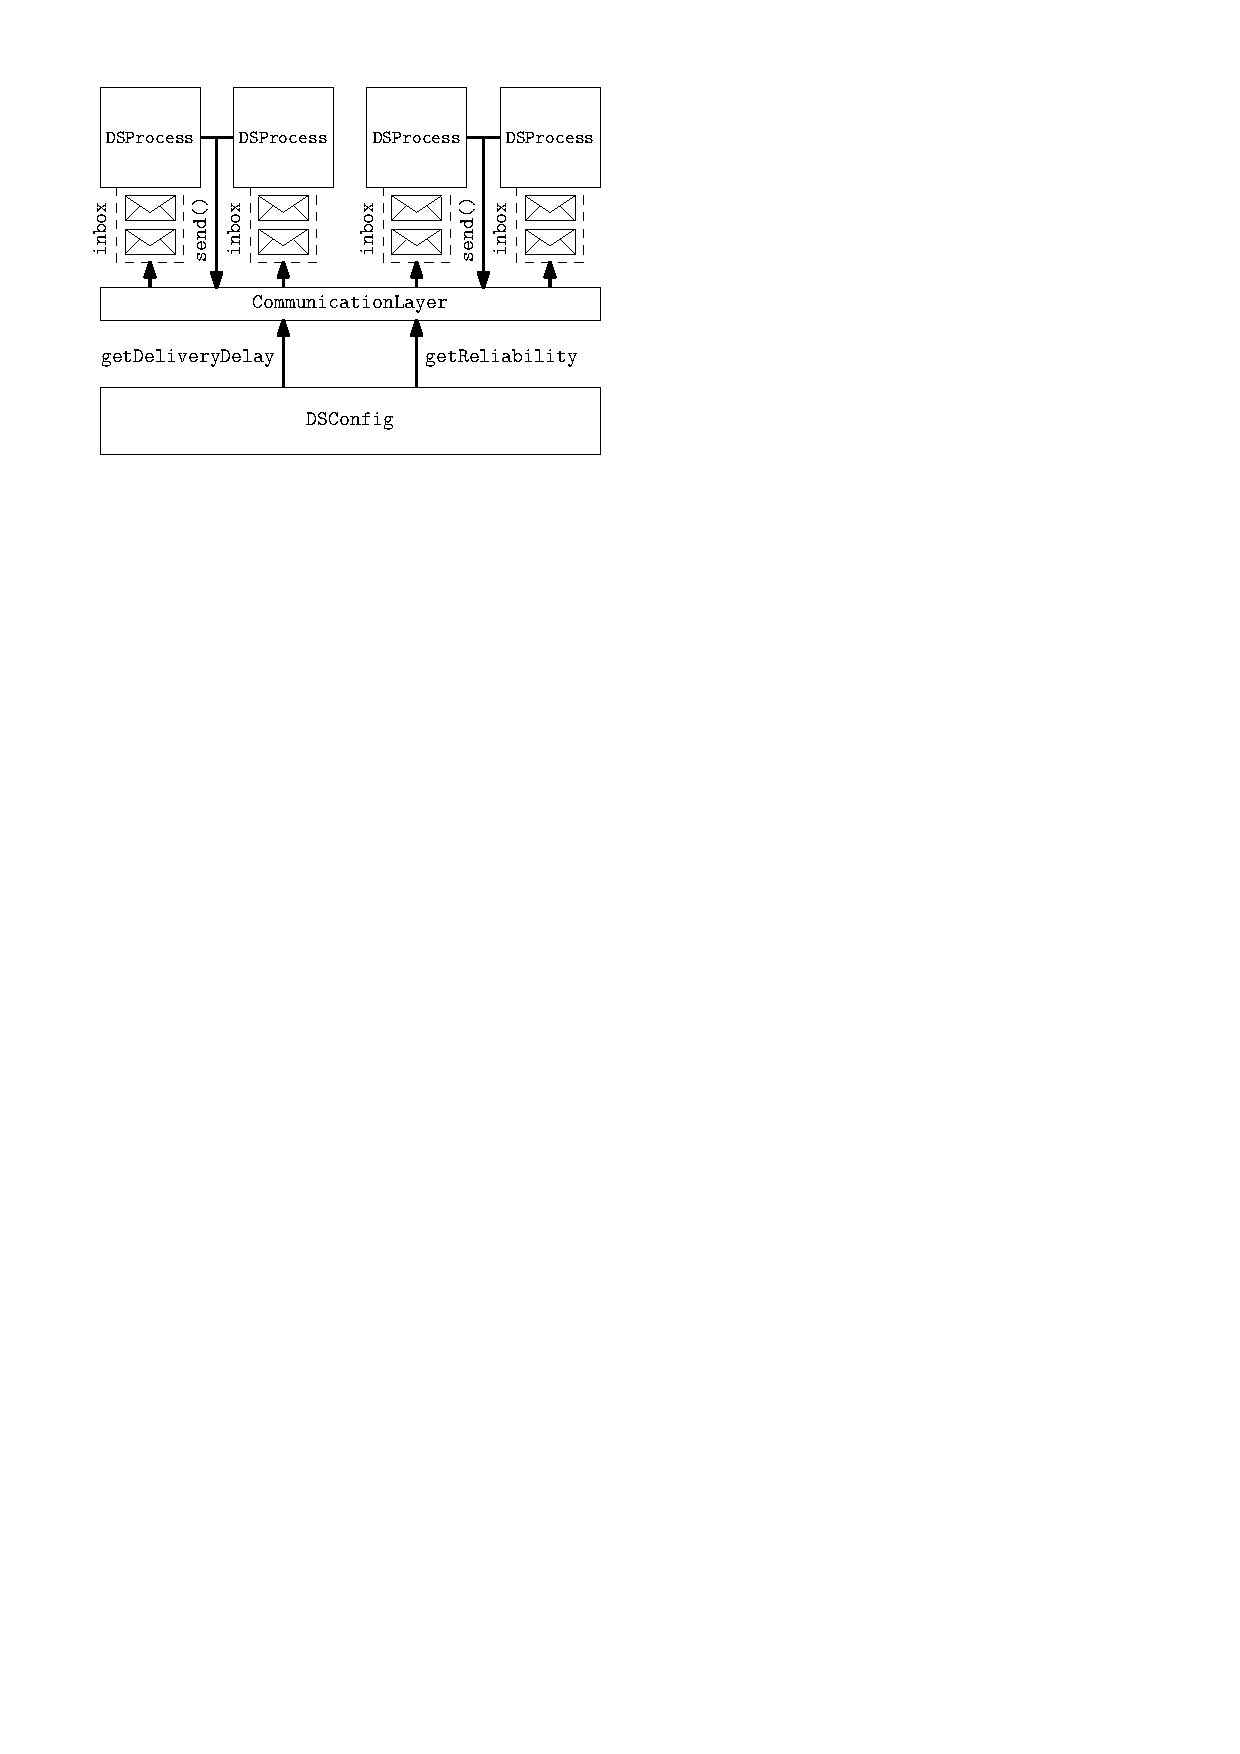
\includegraphics[width=0.9\linewidth]{figs/dsand2.pdf}}%
    \only<3>{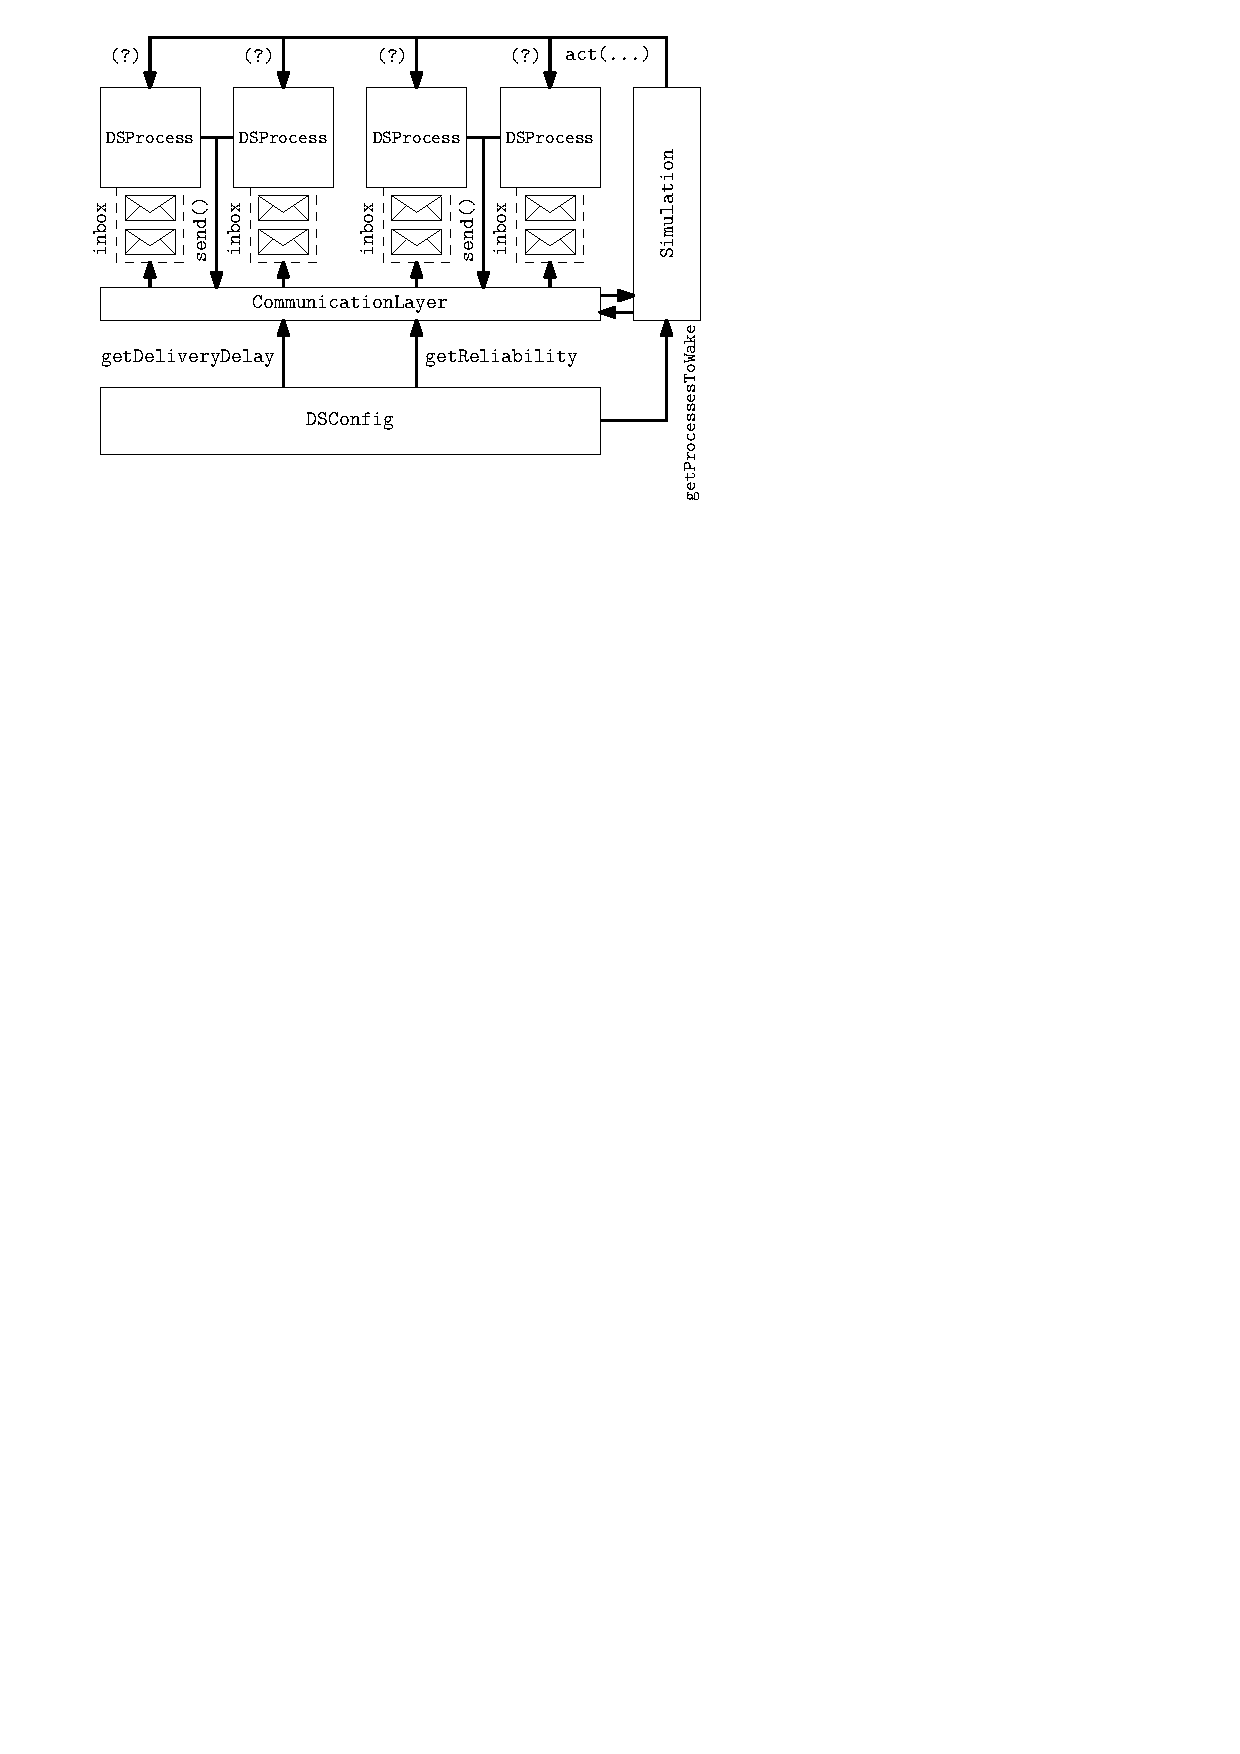
\includegraphics[width=0.9\linewidth]{figs/dsand3.pdf}}%
  \end{center}
  \vspace{-0.5em}
  {\small\see{\url{https://cw.fel.cvut.cz/wiki/courses/b4b36pdv/dsand}}}
\end{frame}

{\setbeamertemplate{frame footer}{\see{{\tt demo/Main.java} \sep {\tt Run demo/Main.java}}}
\begin{frame}[fragile]
\frametitle{Jednoduchá výměna zpráv}

  \begin{block}{Seznamte se s frameworkem DSand}
    Spusťte hlavní třídu \texttt{demo.Main} a vyzkoušejte si framework DSand.
    Můžete si i zkusit změnit parametry systému ve třídě \texttt{demo.DSConfig} a pozorovat, jaký vliv tato změna má na chování distribuovaného systému.
  \end{block}

\end{frame}
}

\section{Synchronní distribuovaný systém}

\begin{frame}
\frametitle{Synchronní distribuovaný systém}

Uvažujme na začátek ideální distribuovaný systém...
\hspace{10pt}\begin{itemize}
  \item Zprávy se nám {\bf neztrácí} a jsou doručované po konstantní době
  \item Procesy nehavarují a pracují {\bf synchronně} (probouzí se všichni naráz)
\end{itemize}

\vspace{2em}\pause
\begin{center}
\Large To je ještě optimističtější předpoklad,\\ než jsme měli v paralelizaci!
\end{center}

\end{frame}

\begin{frame}
\frametitle{Synchronní prohledávání do šířky}

Hledáme nejkratší cestu do cíle.

\begin{itemize}
\item Stavový prostor je silně souvislý
\item Neznáme dopředu velikost ani strukturu prostoru
\end{itemize}

  \pause\vspace{1em}\hrule\vspace{1em}

  \begin{center}
  Jak namapujeme stavový prostor na procesy v síti?
  \end{center}
  \pause
  \begin{itemize}
\item[$\rightarrow$] Každý stav je {\bf samostaný proces}.
\item[$\rightarrow$]  Každý proces zná jen své následovníky.
\item[$\rightarrow$] Jeden z procesů je {\bf kořen}.
\end{itemize}

\hfill Kořen lze zvolit pomocí volby leadera!

\end{frame}

\begin{frame}
\begin{center}
\only<1>{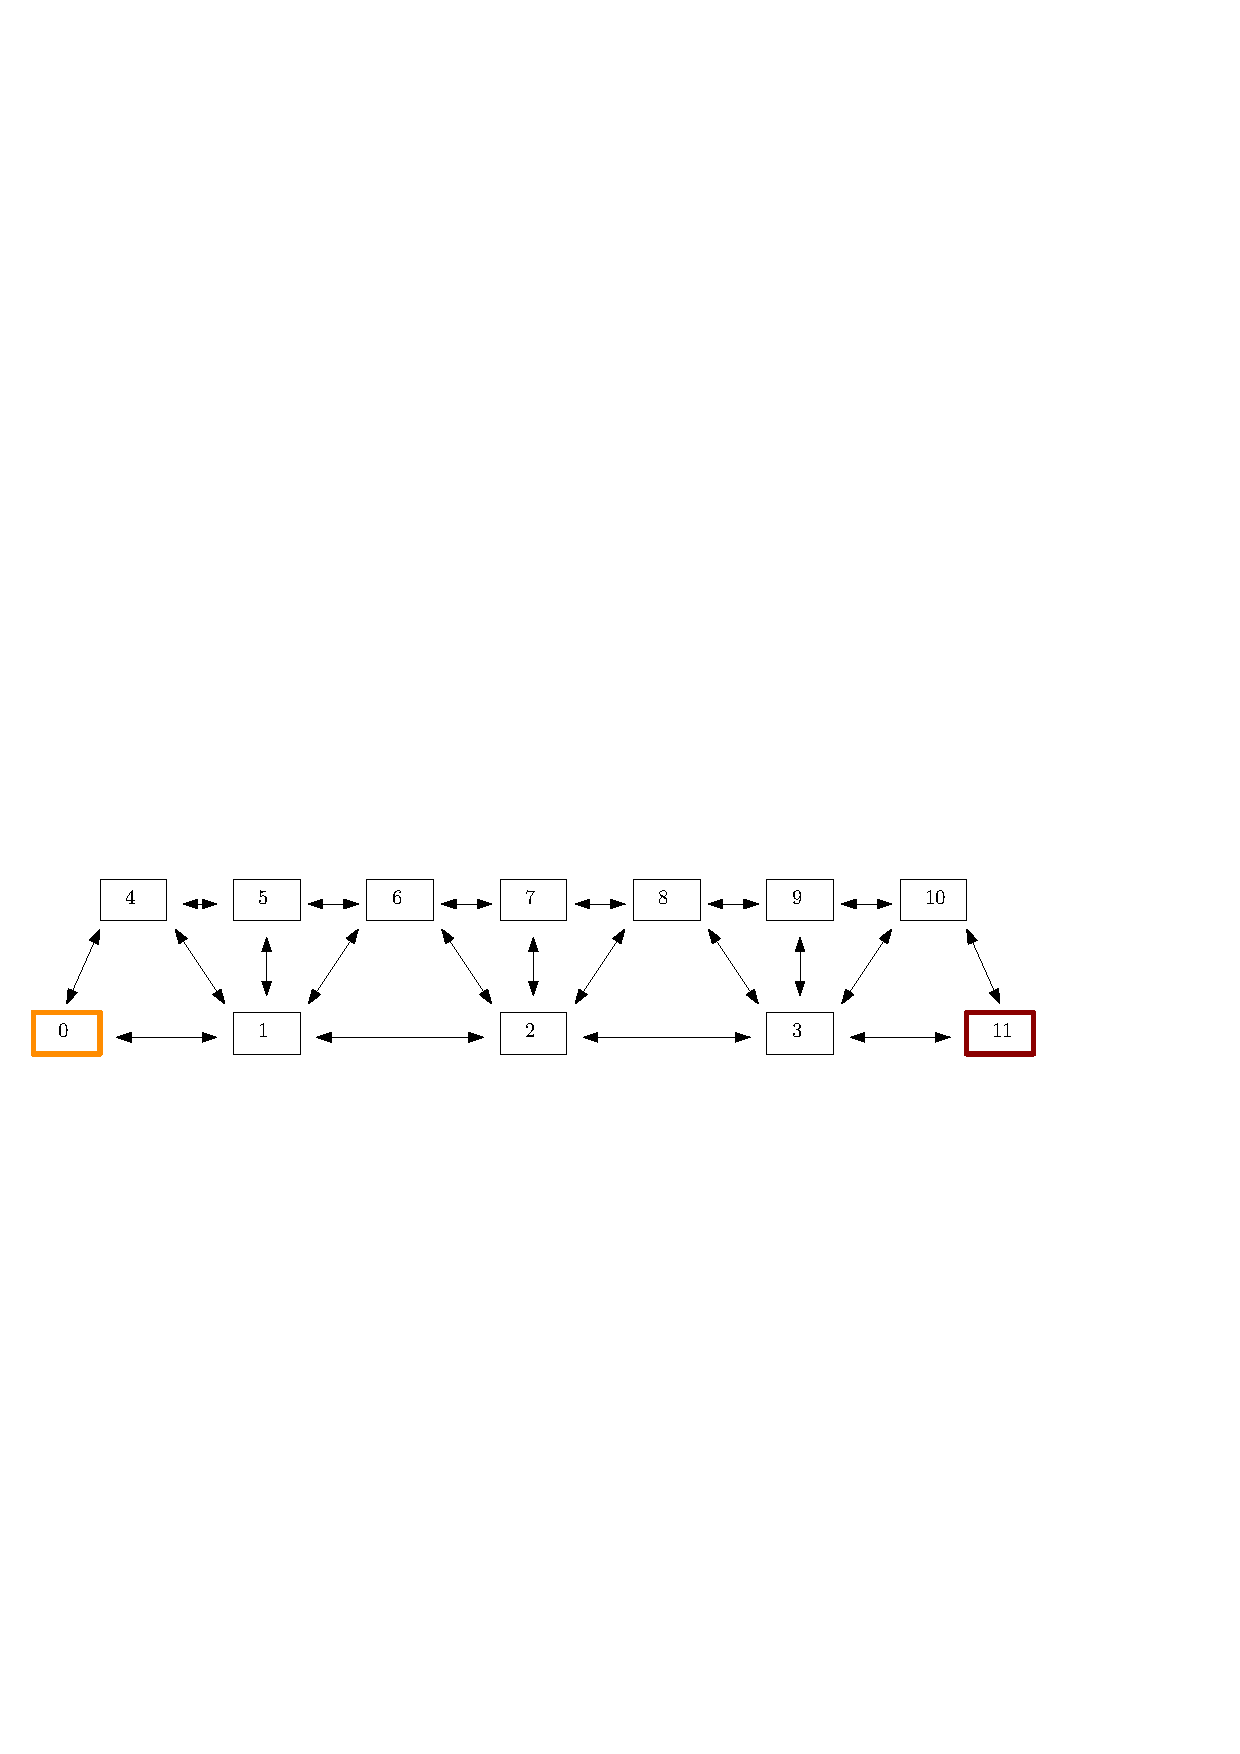
\includegraphics[width=.8\linewidth]{figs/bfs01.pdf}}%
\only<2>{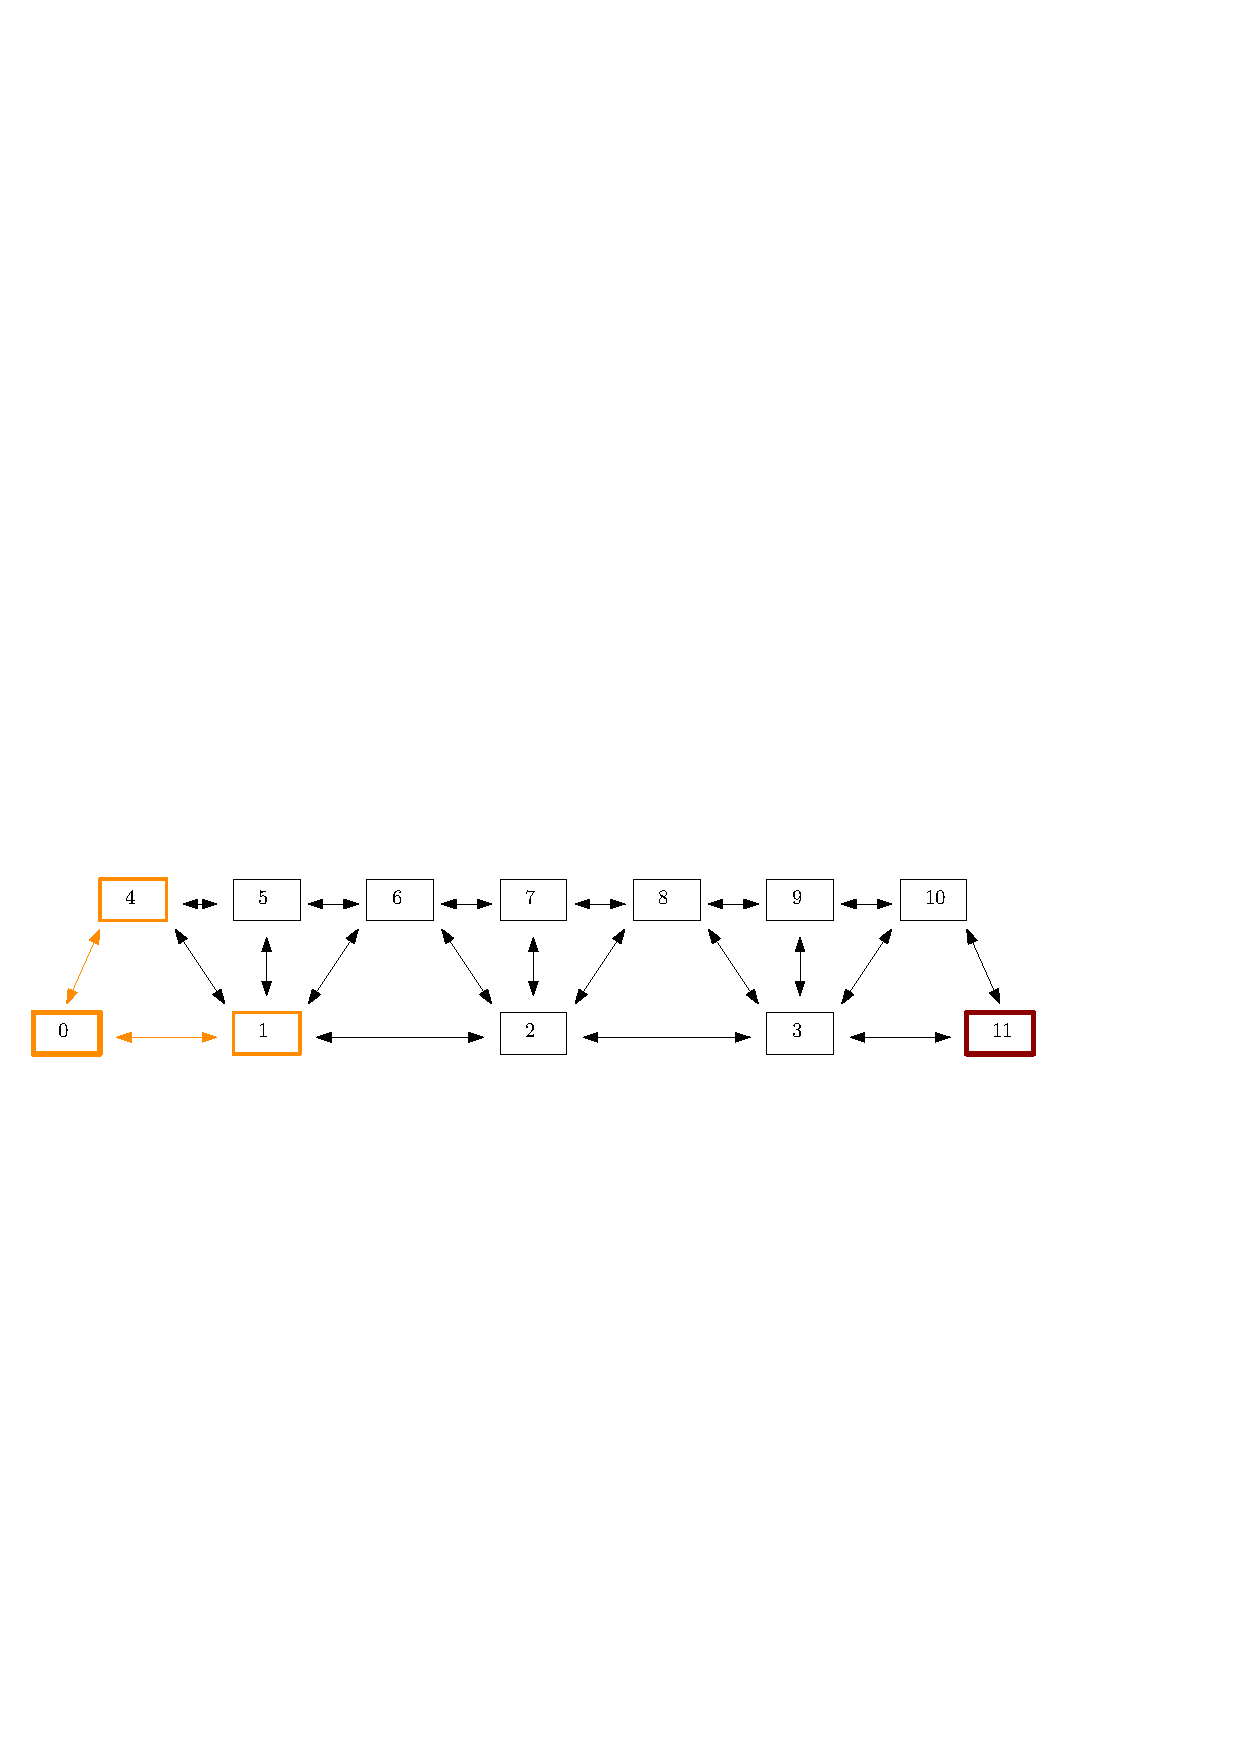
\includegraphics[width=.8\linewidth]{figs/bfs02.pdf}}%
\only<3>{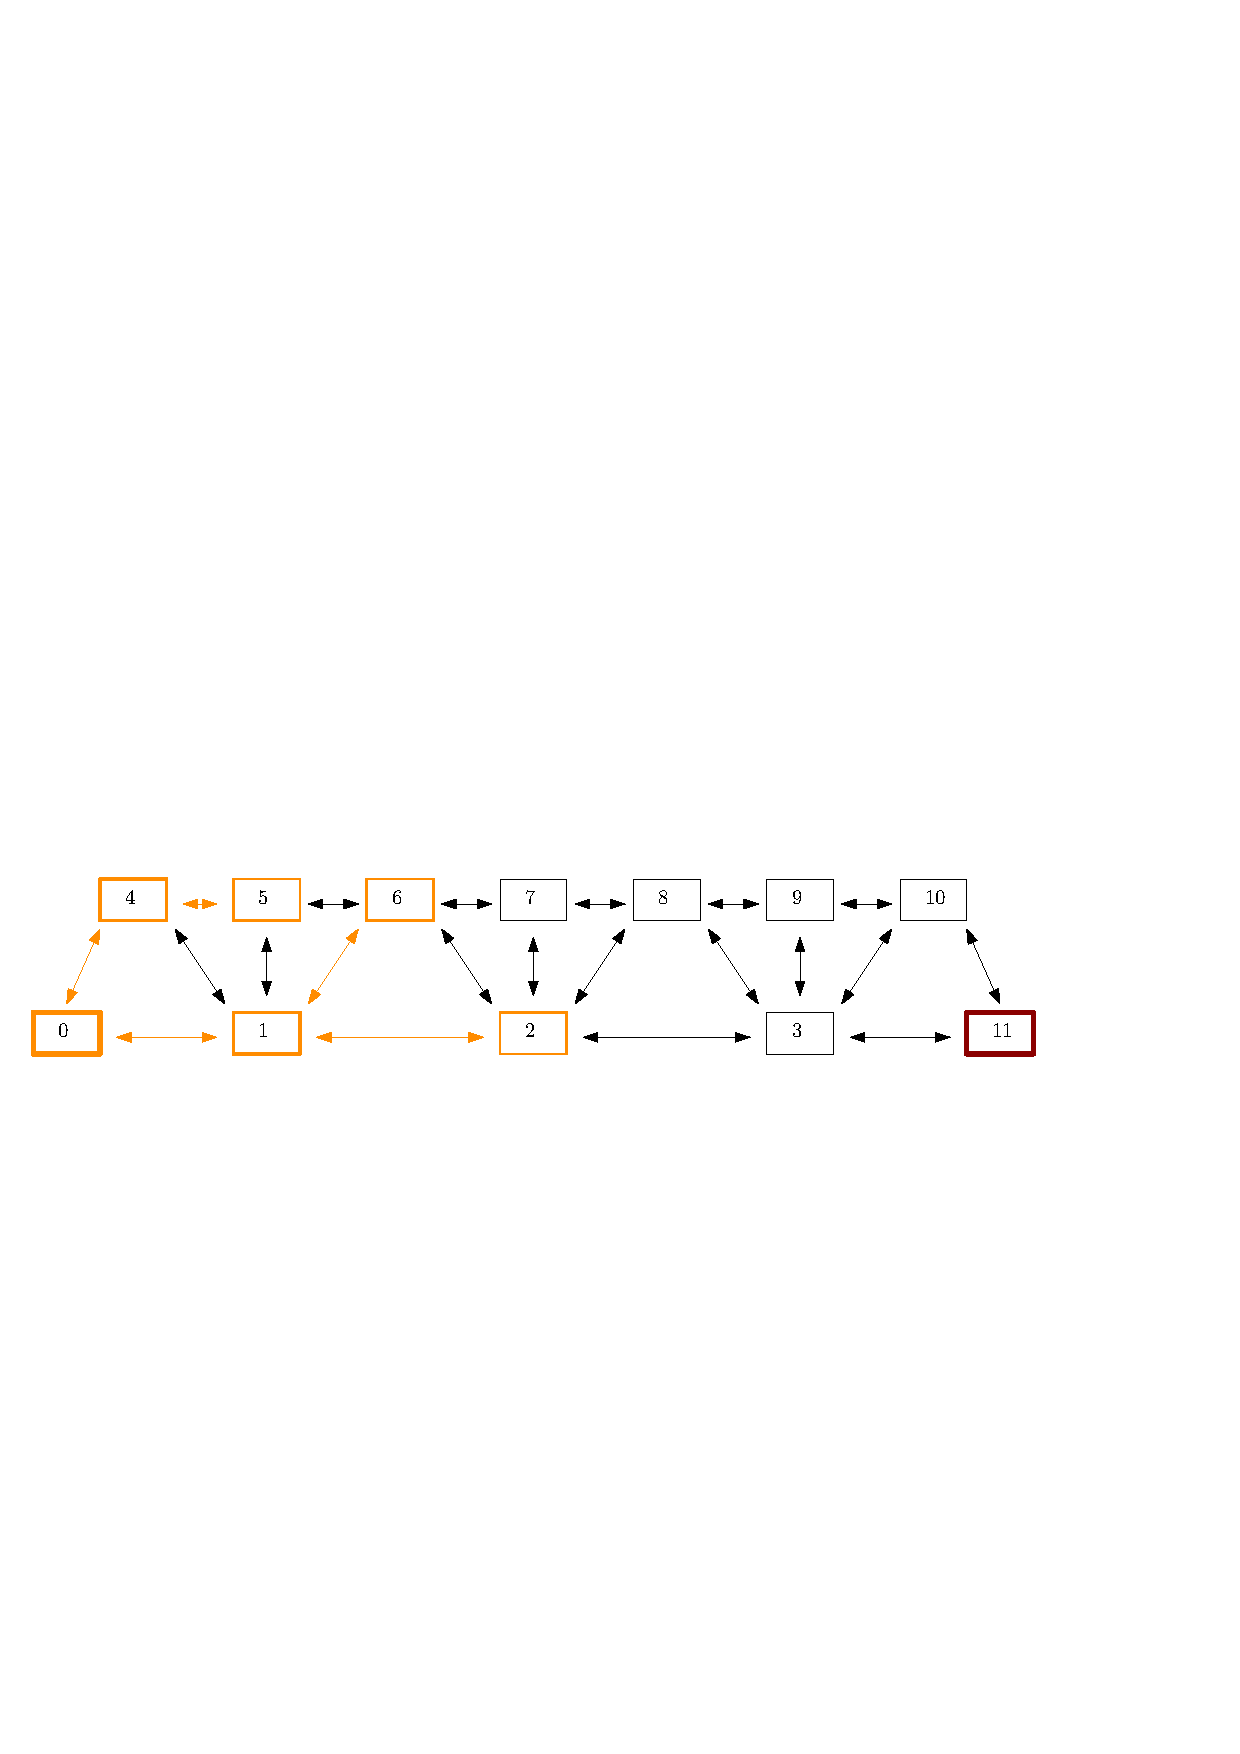
\includegraphics[width=.8\linewidth]{figs/bfs03.pdf}}%
\only<4>{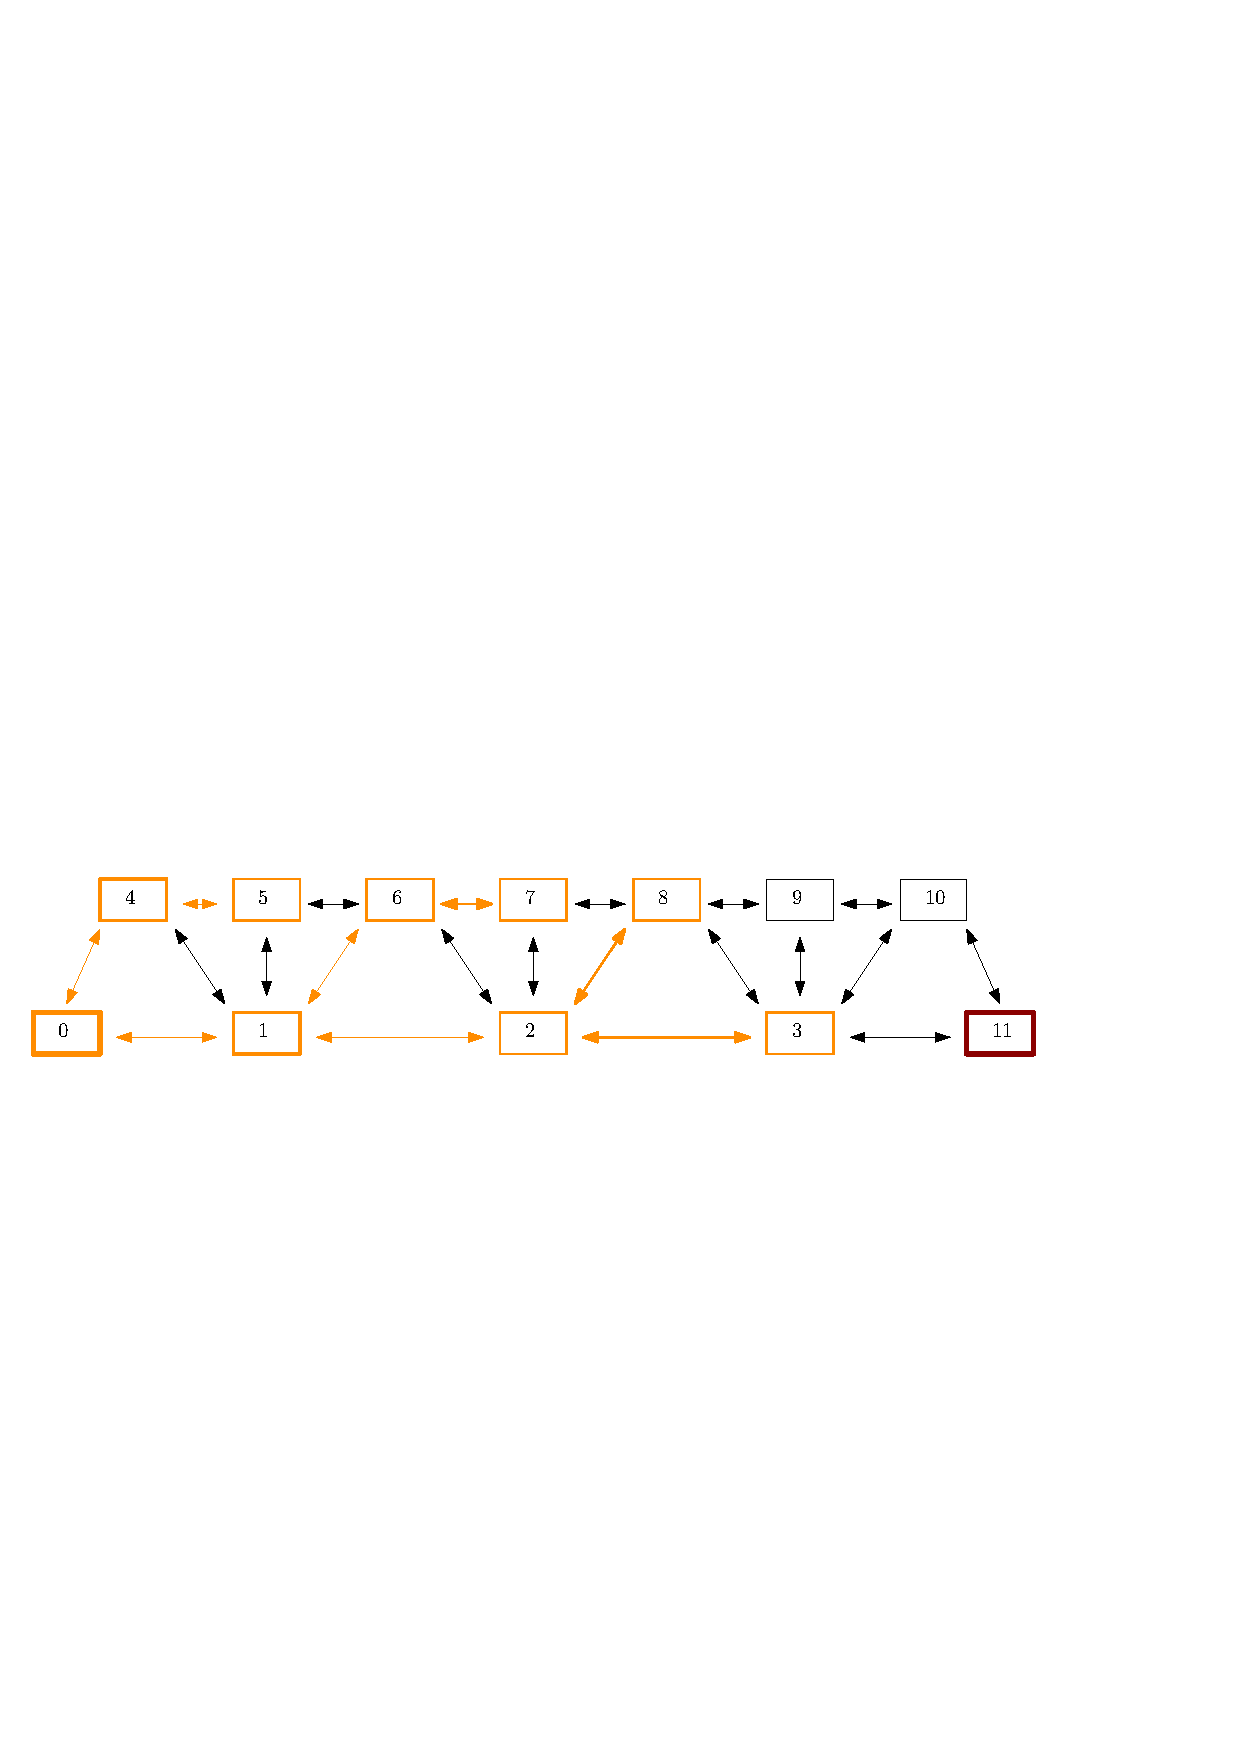
\includegraphics[width=.8\linewidth]{figs/bfs04.pdf}}%
\only<5>{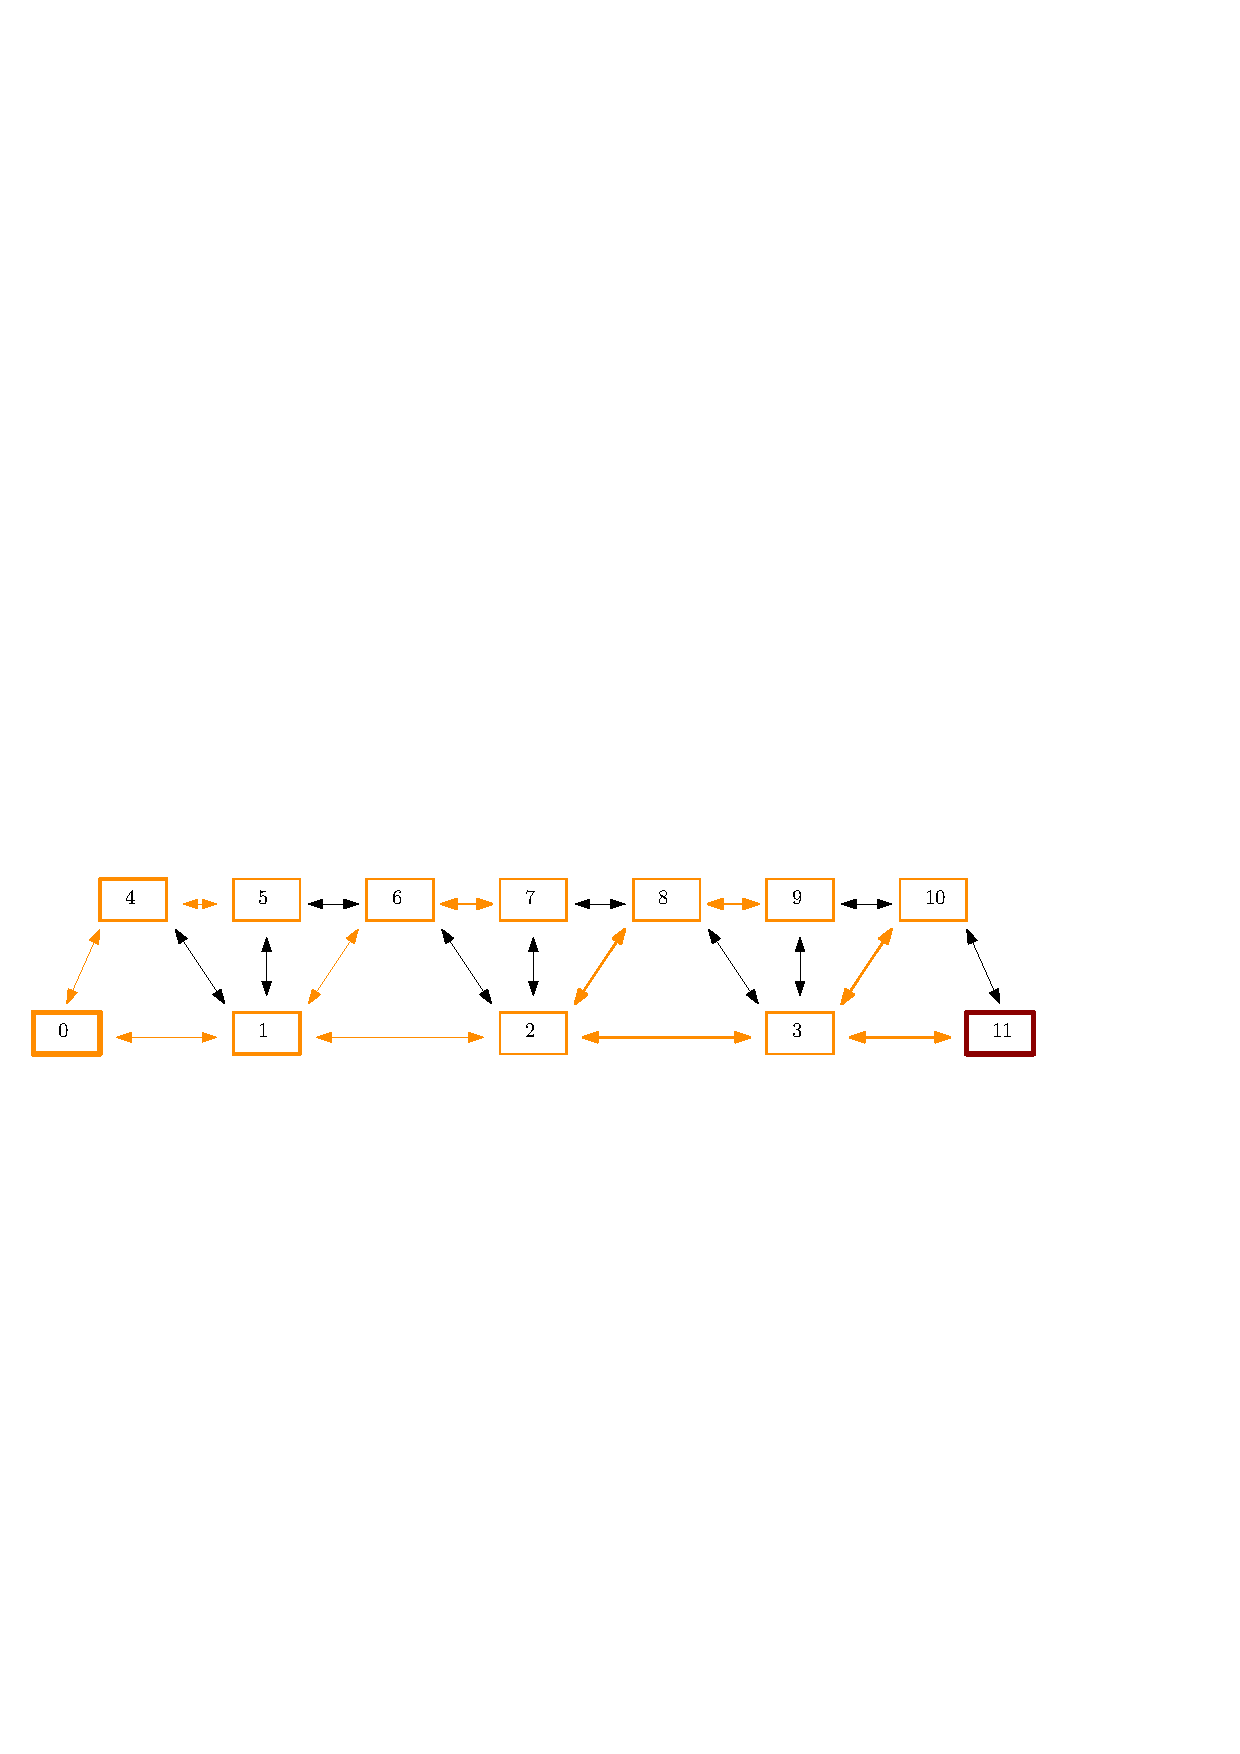
\includegraphics[width=.8\linewidth]{figs/bfs05.pdf}}%
\end{center}
\end{frame}

\begin{frame}
\frametitle{Synchronní prohledávání do šířky}

\begin{center}
Jaký algoritmus bude provádět každý proces?
\end{center}

  \pause\vspace{1em}\hrule\vspace{1em}

Označujeme procesy, když jsou {\bf poprvé navštíveny}
\begin{itemize}
\item Na začátku je označený jen kořen
\item Kořen pošle zprávu \texttt{hledej} všem svým následovníkům
\end{itemize}
\pause
V každém kole \textit{neoznačené} procesy, které přijmou zprávu \texttt{hledej}, provedou
\begin{itemize}
\item Označí se
\item Určí jednoho z procesů, od kterého přijal zprávu, jako předka
\item Pošlou zprávu \texttt{hledej} všem svým následovníkům
\end{itemize}



\end{frame}

\begin{frame}

\begin{center}
\only<1>{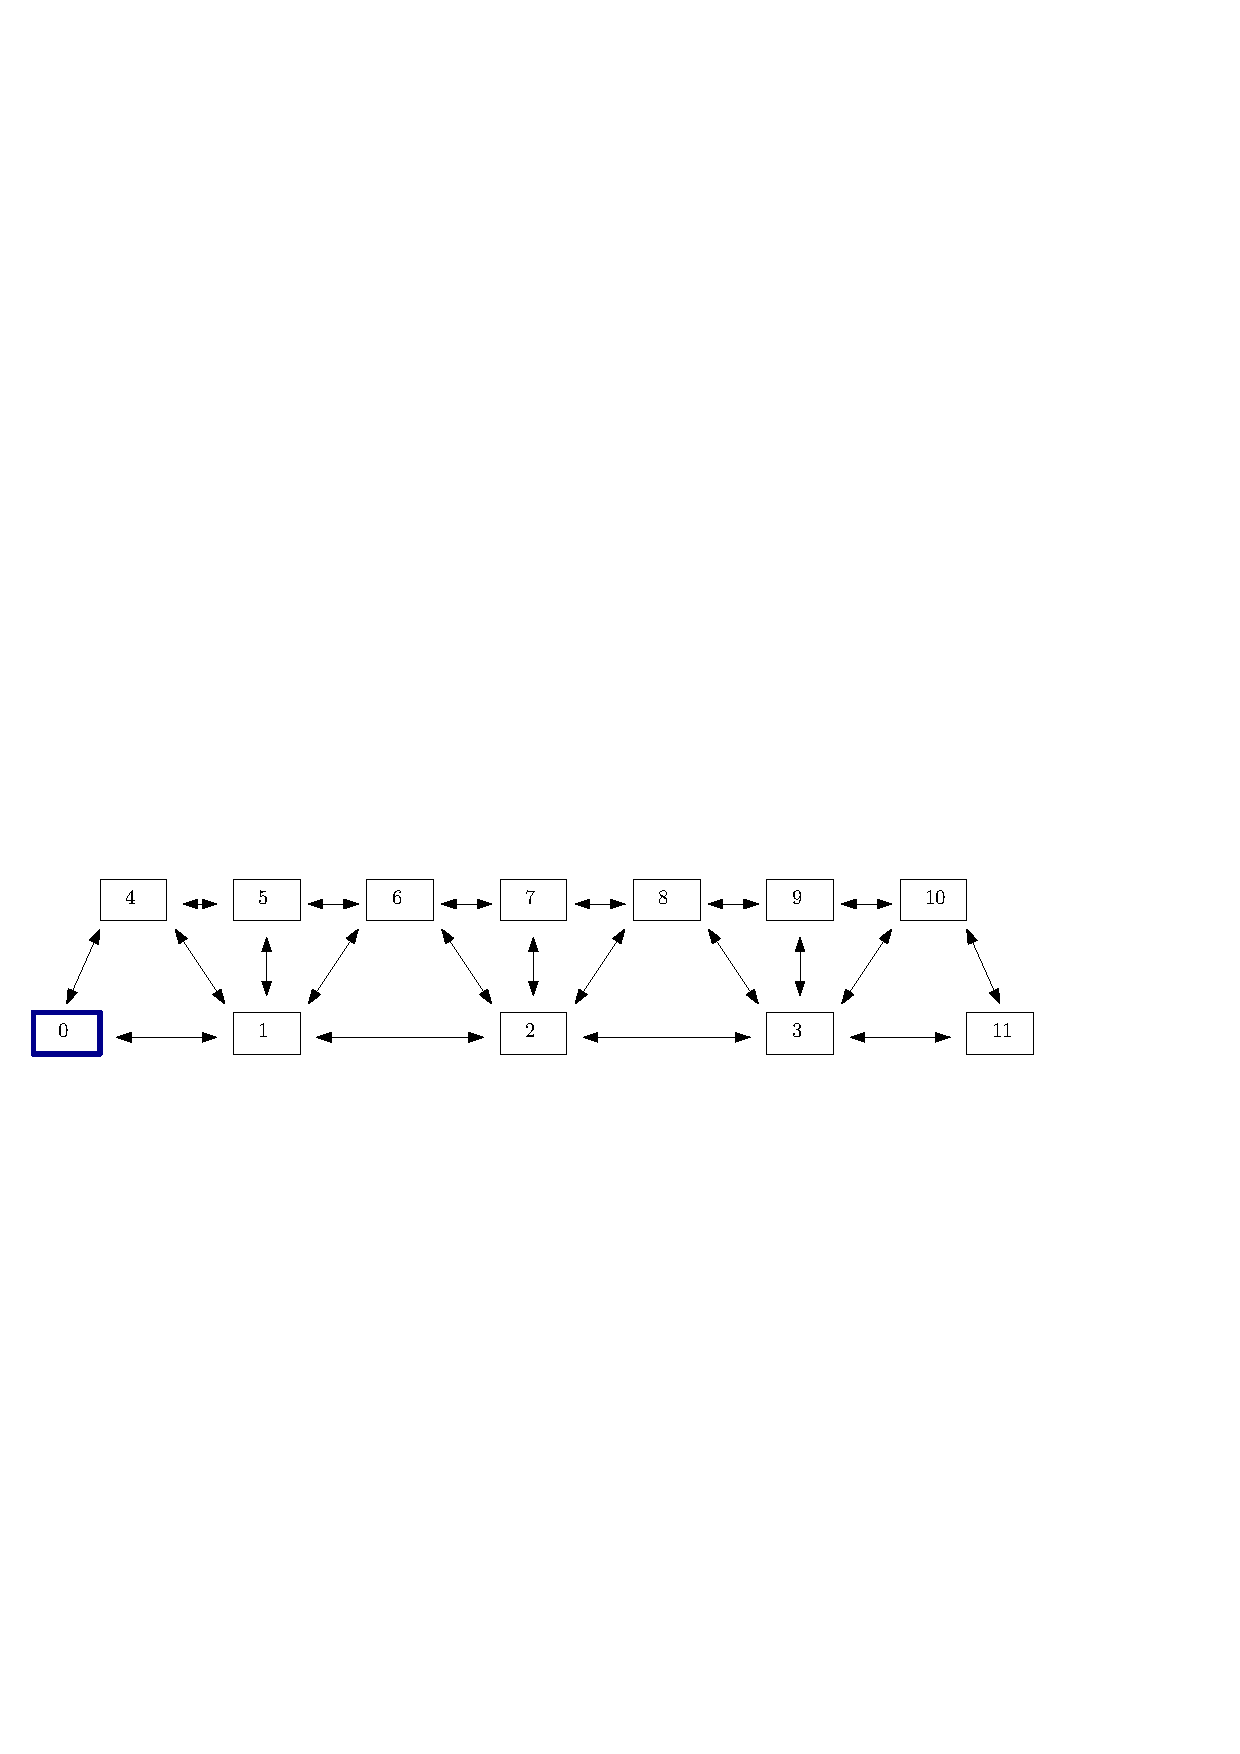
\includegraphics[width=.8\linewidth]{figs/dbfs01.pdf}}%
\only<2>{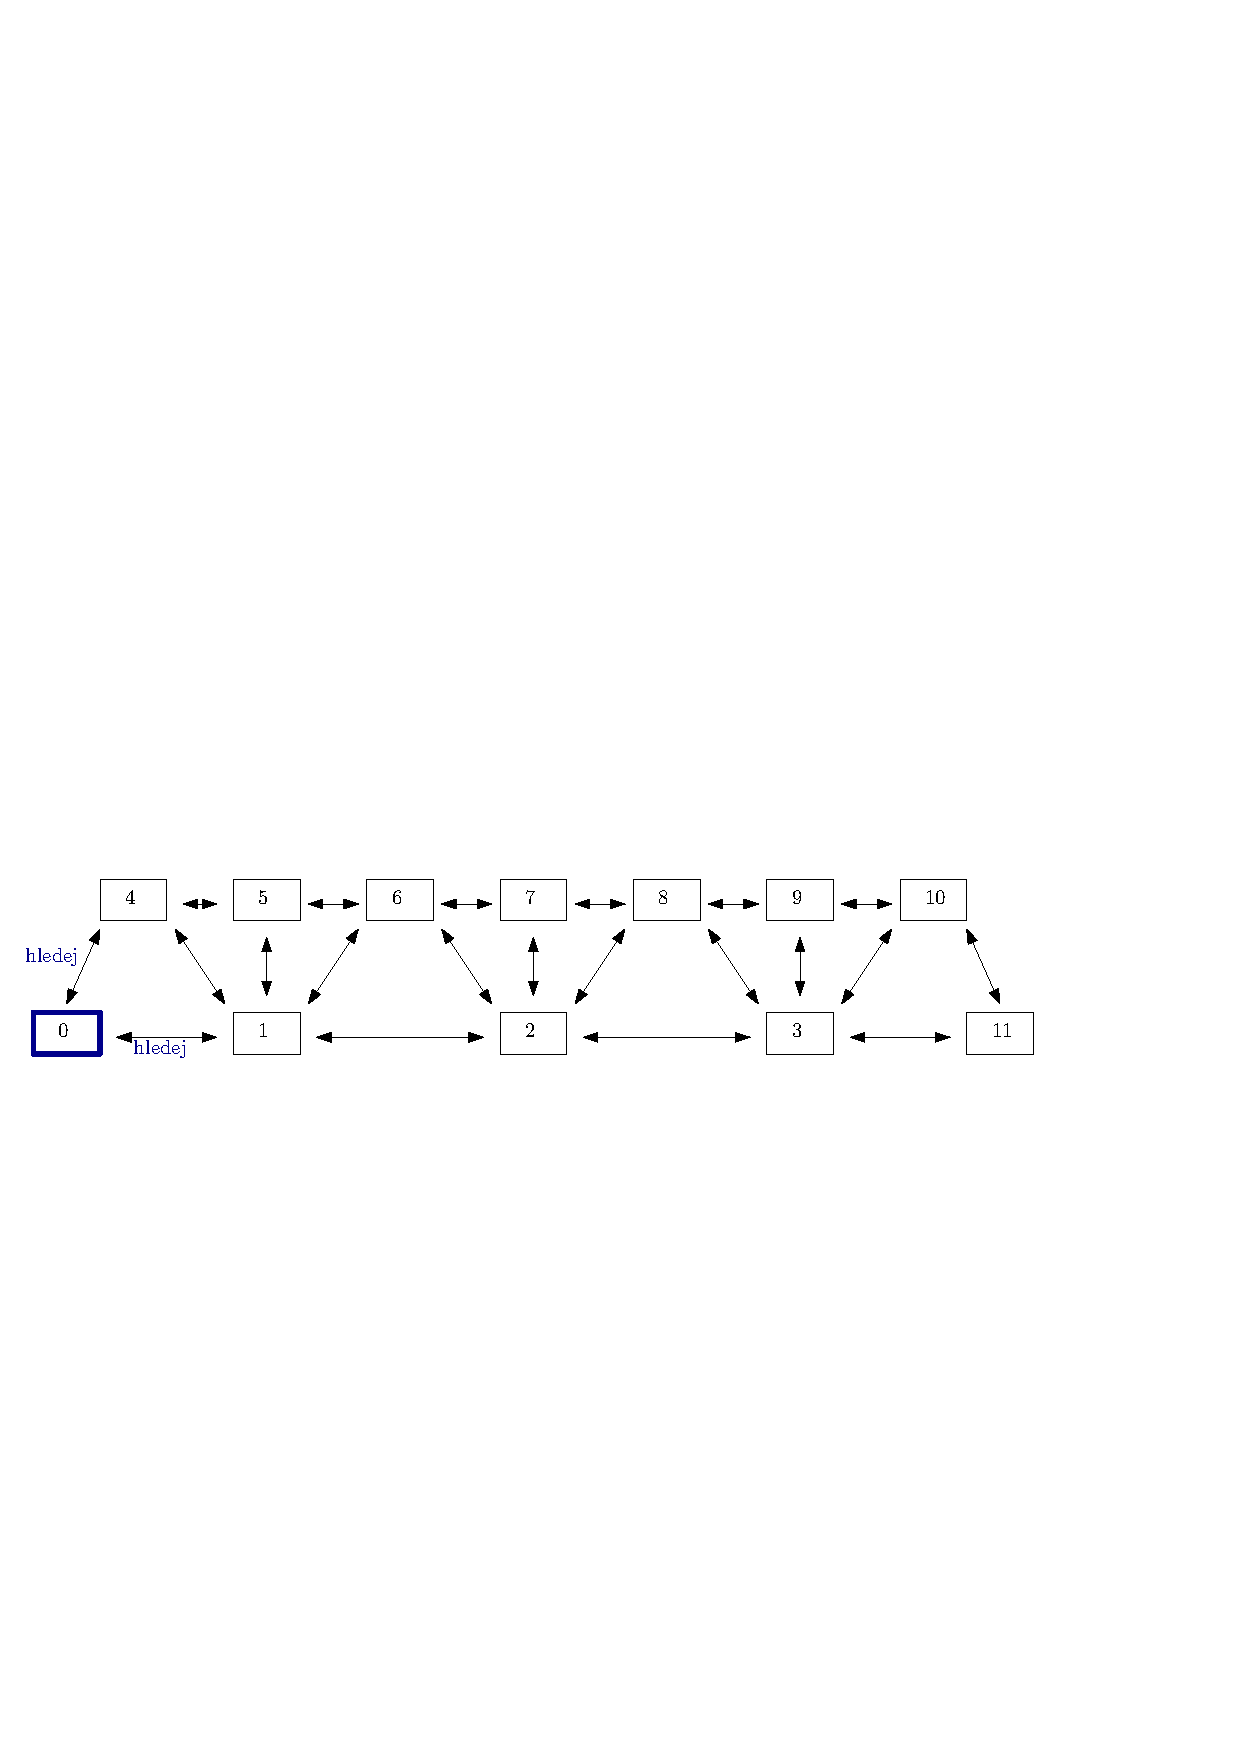
\includegraphics[width=.8\linewidth]{figs/dbfs02.pdf}}%
\only<3>{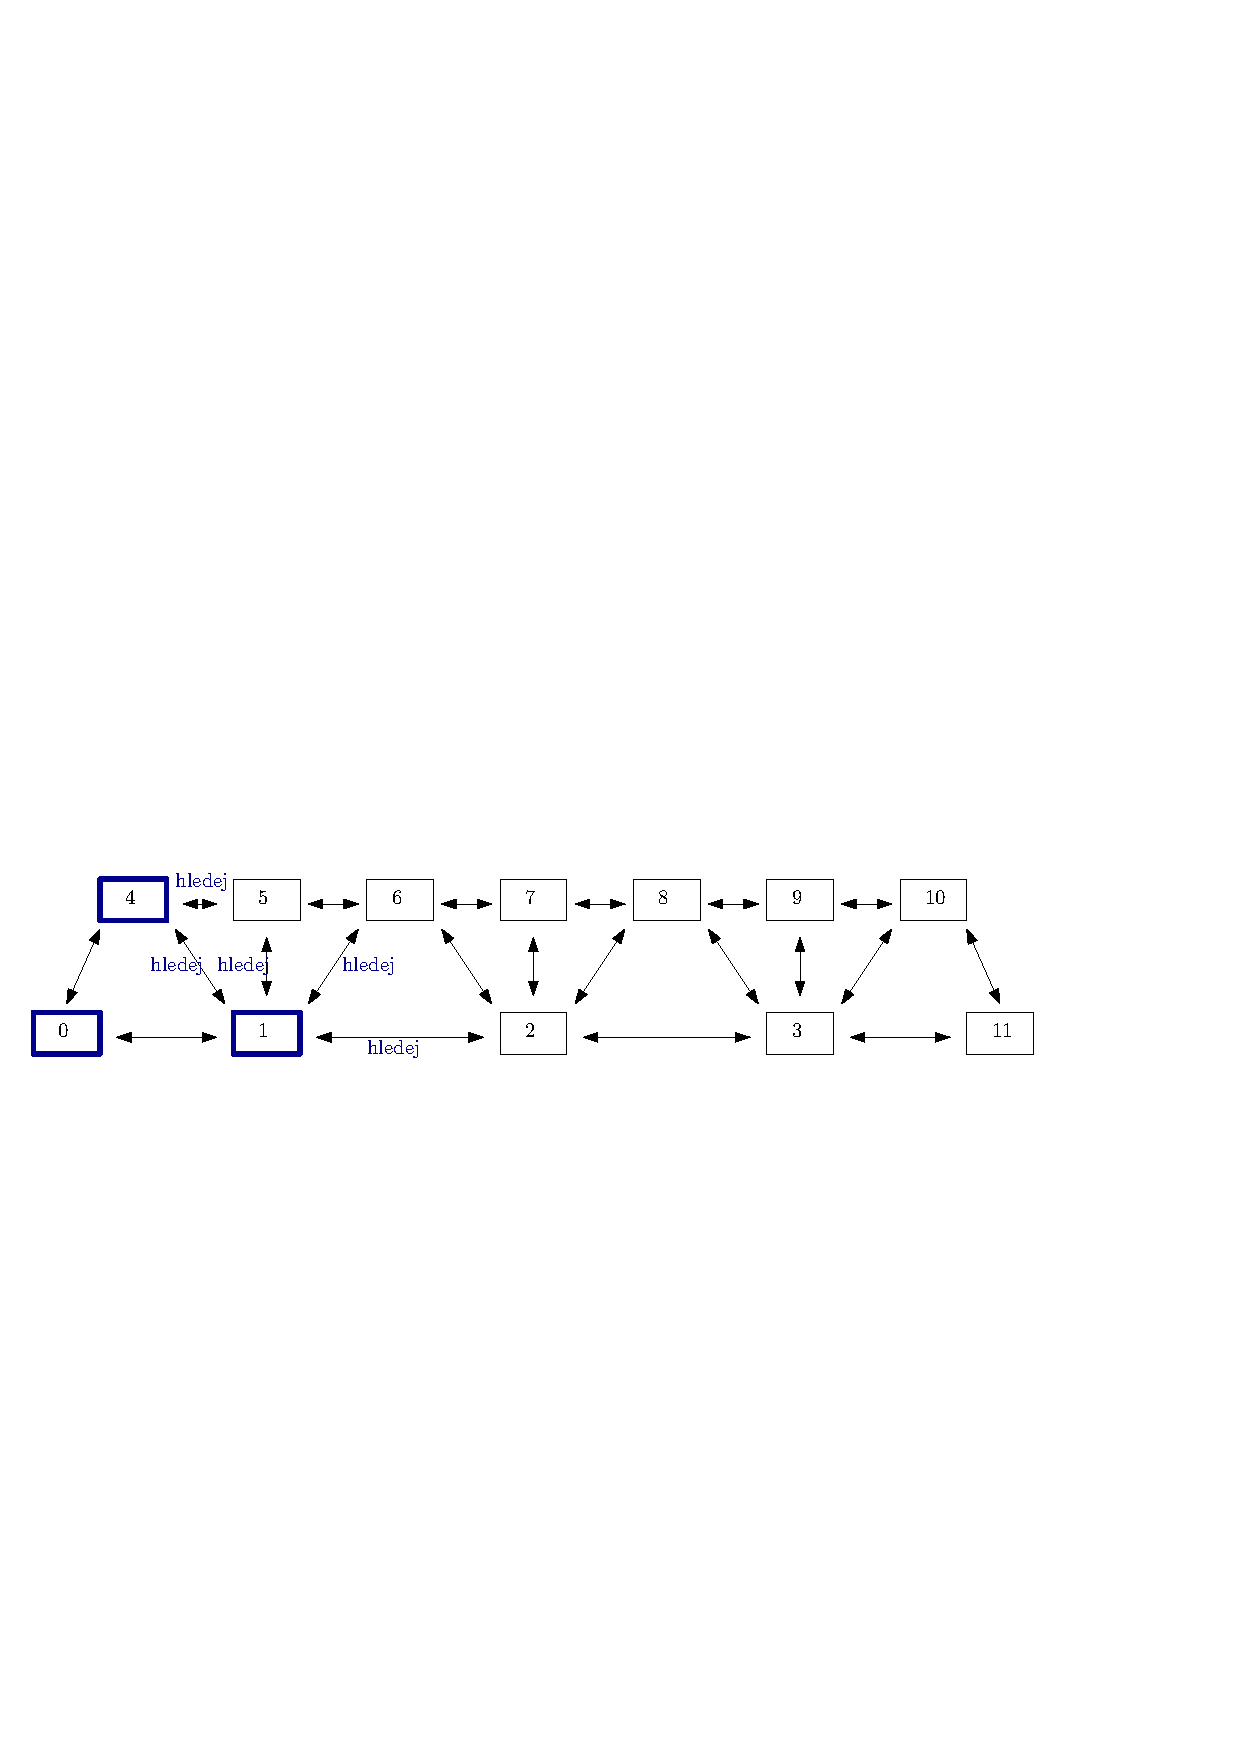
\includegraphics[width=.8\linewidth]{figs/dbfs03.pdf}}%
\only<4>{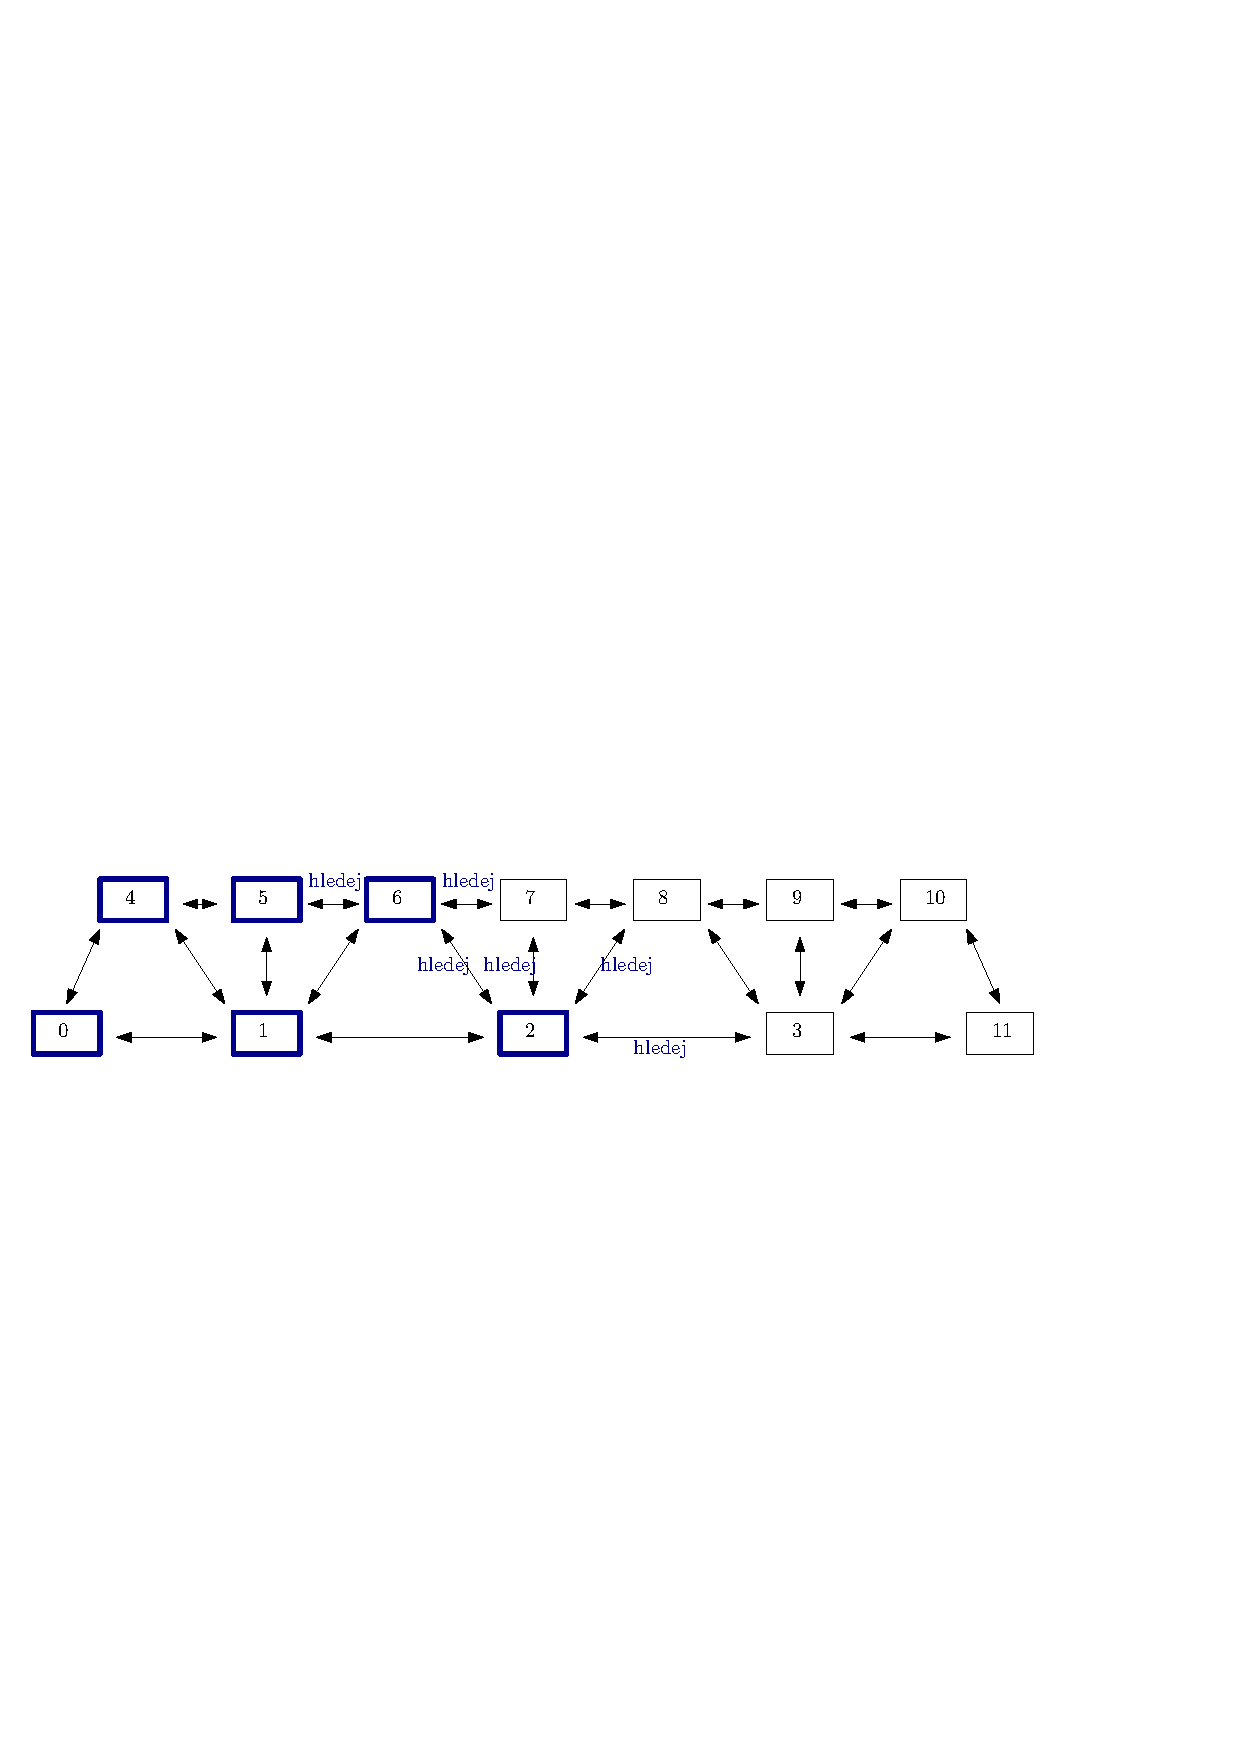
\includegraphics[width=.8\linewidth]{figs/dbfs04.pdf}}%
\end{center}
\end{frame}

{\setbeamertemplate{frame footer}{\see{{\tt bfs/BFSProcess.java} \sep {\tt Run bfs/SynchronousAndReliable.java}}}
\begin{frame}[fragile]
\frametitle{Synchronní prohledávání do šířky}

  \begin{block}{Naimplementujte distribuované prohledávání do šířky}
    Do souboru \texttt{BFSProcess.java} doplňte kód procesů, které budou prohledávat síť do šířky. Předpokládejte, že systém je synchronní. Ve chvíli kdy najdete cíl, ukončete celý distribuovaný výpočet pomocí metody \texttt{terminateAll(...)}.
  \end{block}

\end{frame}
}

\begin{frame}

\begin{center}
\Large Jak vypsat posloupnost procesů na cestě k cíli?
\end{center}

\pause\vspace{0.8em}

\hfill Propagujeme informaci napříč sítí!


\end{frame}

{\setbeamertemplate{frame footer}{\see{{\tt bfs/BFSProcess.java} \sep {\tt Run bfs/SynchronousAndReliable.java}}}
\begin{frame}[fragile]
\frametitle{Synchronní prohledávání do šířky s předáváním cesty}

  \begin{block}{Doimplementujte konstrukci cesty z kořene do cíle}
    Přidejte do Vašeho algoritmu pro distribuované prohledávání zpětnou rekonstrukci cesty z cíle do kořenu. Ve chvíli kdy kořen bude znát celou cestu, vypište ji a ukončete distribuovaný výpočet.
  \end{block}

\end{frame}
}

{\setbeamertemplate{frame footer}{\see{{\tt bfs/BFSProcess.java} \sep {\tt Run bfs/SlowOptimalPath.java},\quad {\tt Run bfs/FailingNode2.java}}}
\begin{frame}
\begin{center}
\Large Jak bude tento algoritmus fungovat, když systém nebude synchronní?
\end{center}

 \pause\vspace{2em}

  \begin{block}{Vyzkoušejte nesynchronní scénáře}
    Zkuste spustit scénáře \texttt{SlowOptimalPath.java}, ve kterém jsou zprávy pouze po optimální cestě zpožděny a \texttt{FailingNode2.java}, kdy se zprávy procesu 2 ztrácí. Jaké jsou výsledky jednotlivých scénářů?
  \end{block}

  \pause\vspace{2em}

\faWarning \hspace{3pt}
  \textbf{Nemáme žádné garance.} Výsledek nemusí být optimální, dokonce ani nemusí nikdy doběhnout.

\end{frame}
}

% Frame with the feedback QR code 
\framefeedback{}

\end{document}
